Este capítulo tem como objetivo apresentar os resultados obtidos pelos procedimentos descritos no
Capítulo~\ref{metodologia}.
Serão avaliados se os objetivos foram atingidos e serão ressaltados problemas encontrados no desenvolvimento.

\section{Primeira Etapa}

A primeira etapa consiste no treinamento de algoritmos de aprendizado de máquina a partir de base de dados anotada
ruidosamente, replicando assim o trabalho de Go \textit{et al.}
Nesta fase foram utilizados o dados disponibilizados no Sentiment140 para treinamento e teste do algoritmo.
Entretanto, o baixo número de exemplos pode causar pequenas variações nos resultados obtidos.

Para seleção de hiperparâmetros foram treinados modelos de Naïve Bayes com diferentes fatores de regularização por
suavização de distribuição de Laplace de maneira a encontrar o ponto de melhor performance.
O parâmetro selecionado foi o que obteve maior valor médio de acurácia entre 10 partições de validação cruzada.
A Figura~\ref{fig:go_nb} mostra a acurácia obtidas por diferentes valores de regularização nos grupos de validação.
O eixo horizontal da Figura~\ref{fig:go_nb} corresponde aos valores variados de suavização de Laplace aplicados, e o
eixo vertical contém a acurácia correspondente a cada um destes valores, as barras de erro correspondem a um desvio
padrão da validação cruzada.
A linha vertical vermelha presente na Figura~\ref{fig:go_nb} indica o parâmetro selecionado, aproximadamente 4,1, que
foi escolhido por obter maior média de acurácia na validação cruzada, 78,2\%.
Uma vez decidido o parâmetro de regularização, o modelo foi retreinado, dessa vez utilizando todos os dados do conjunto
de treinamento.
Aplicando-se este modelo no conjunto de teste foi obtida acurácia de 83,3\%, este valor se aproxima ao apresentado por Go
\textit{et al.}: 81,3\%.

\begin{figure}
\begin{center} {
    \begin{center}
    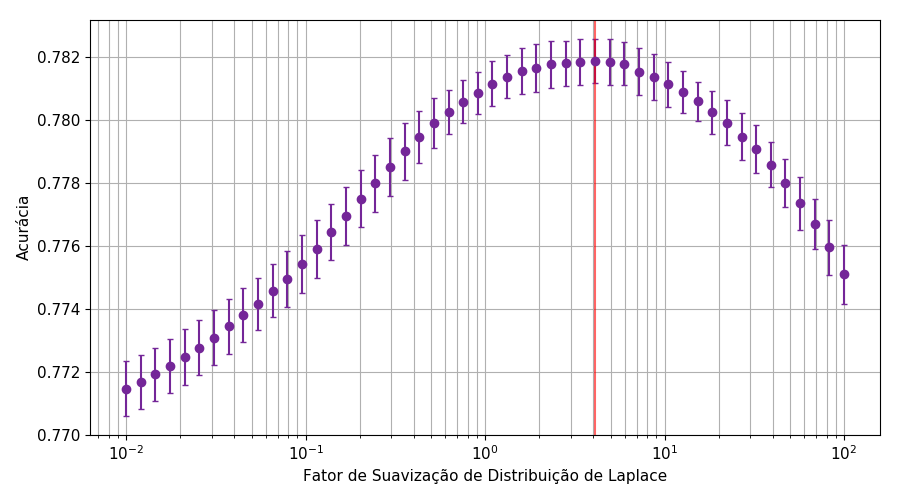
\includegraphics[scale=0.5]{go_nb.png}
    \caption{Seleção de hiperparâmetros de Naïve Bayes - Etapa 1.}
    \label{fig:go_nb}
    \end{center}
}
\end{center}
\end{figure}

A seleção do parâmetros do modelo formado por \textit{Support Vector Machines} foi feita por processo semelhante ao
anterior.
Foram variados o fator de regularização $L_{2}$, selecionando o modelo de maior acurácia média da validação cruzada.
A Figura~\ref{fig:go_svm} apresenta os resultados obtidos, no qual o fator de $6 \times 10^{-6}$ resultou na acurácia
média de 80.0\% sobre o conjunto de validação e 83,0\% de acurácia no conjunto de teste.

\begin{figure}
\begin{center} {
    \begin{center}
    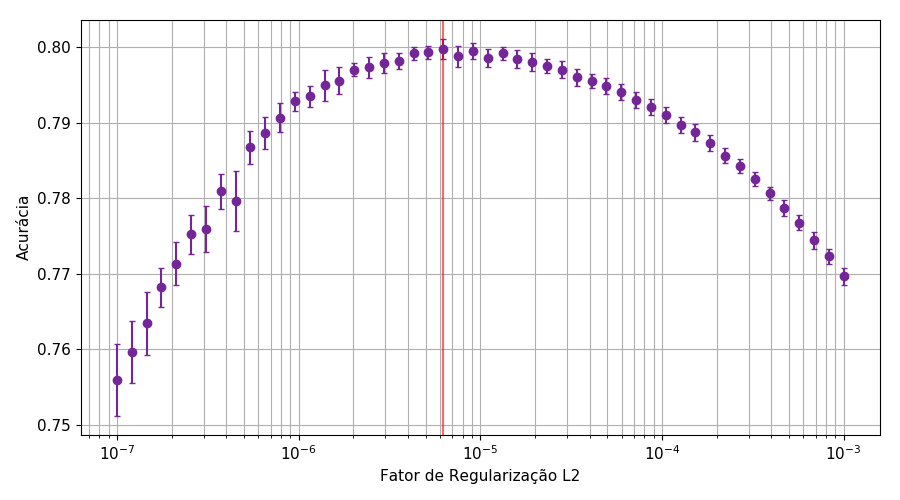
\includegraphics[scale=0.5]{go_svm.png}
    \caption{Seleção de hiperparâmetros de SVM - Etapa 1.}
    \label{fig:go_svm}
    \end{center}
}
\end{center}
\end{figure}

A Tabela~\ref{tab:go_compara} apresenta os resultados obtidos tanto no Sentiment140 quanto pela replicação de
seu método.
Pode se observar que foram atingidos valores próximos a referência, validando assim os pré-processamentos e as
implementações dos algoritmos aplicados.

% Resultados pós calibração
\begin{table}[h]
    \begin{center}
        \begin{tabular}{| l | r | r |}
        \hline
        \textbf{Algoritmo} & \textbf{Original} & \textbf{Replicação} \\ \hline
        Naïve Bayes & 81,3\% & 83,3\% \\ \hline
        \textit{Support Vector Machine} &  82,2\% & 83,0\% \\ \hline
        \end{tabular}
        \caption[Comparação de resultados da replicação dos classificadores do Sentiment140.]{Comparação de resultados da replicação dos classificadores do Sentiment140~\cite{go09}.}
        \label{tab:go_compara}
    \end{center}
\end{table}

\section{Segunda Etapa}

A segunda etapa consiste na validação do processo de formação de base de treinamento por supervisão distante.
A aplicação de técnicas de pré-processamento e algoritmos previamente validados neste novo conjunto de dados visa tanto
comparar o processo de elaboração por anotação ruidosa quanto servir como referência para a aplicação de algoritmos de
\textit{Deep Learning}.
Nesta etapa, os modelos foram avaliados tanto pelo seu desempenho na base de teste disponibilizada por Go
\textit{et al.} quanto aplicado na base de testes formada pela coletânea de \textit{tweets} oferecida pelas conferências
SemEval, como descrito na Seção~\ref{sec:data}

Assim como na fase anterior, foram treinados modelos por Naïve Bayes e \textit{Support Vector Machines}.
Neste caso, a seleção dos parâmetros de regularização foi feita de maneira a maximizar a área sob a curva ROC, visto que
os dados de treinamento apresentam desbalanceamento de classes.
As Figuras~\ref{fig:nb_selecao} e~\ref{fig:svm_selecao} mostram os resultados dos modelos, respectivamente, Naïve Bayes e
SVM a mudanças nos parâmetros de regularização, as linhas verticais vermelhas apontam os parâmetros que obtiveram maior
média de área sob a curva ROC dentre os grupos de validação quando aplicada validação cruzada com 10 partições.

\begin{figure}
\begin{center} {
    \begin{center}
    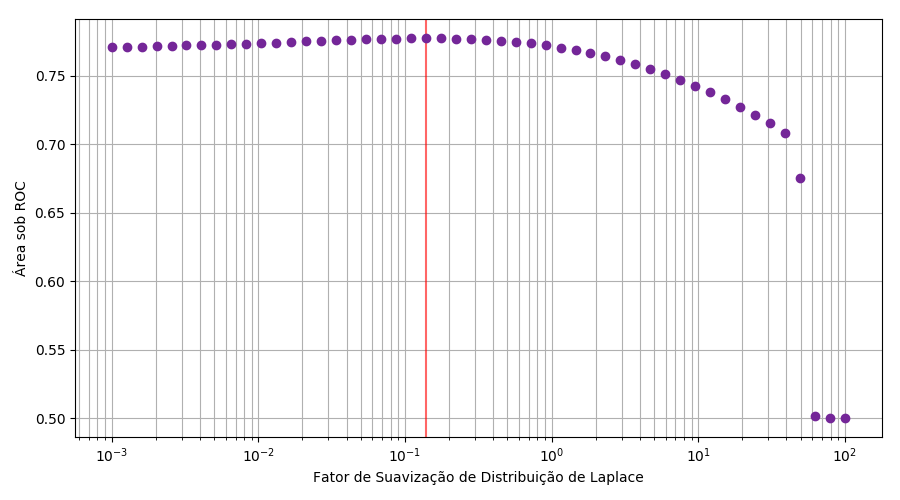
\includegraphics[scale=0.5]{nb_selecao.png}
    \caption{Seleção de hiperparâmetros de Naïve Bayes - Etapa 2.}
    \label{fig:nb_selecao}
    \end{center}
}
\end{center}
\end{figure}

\begin{figure}
\begin{center} {
    \begin{center}
    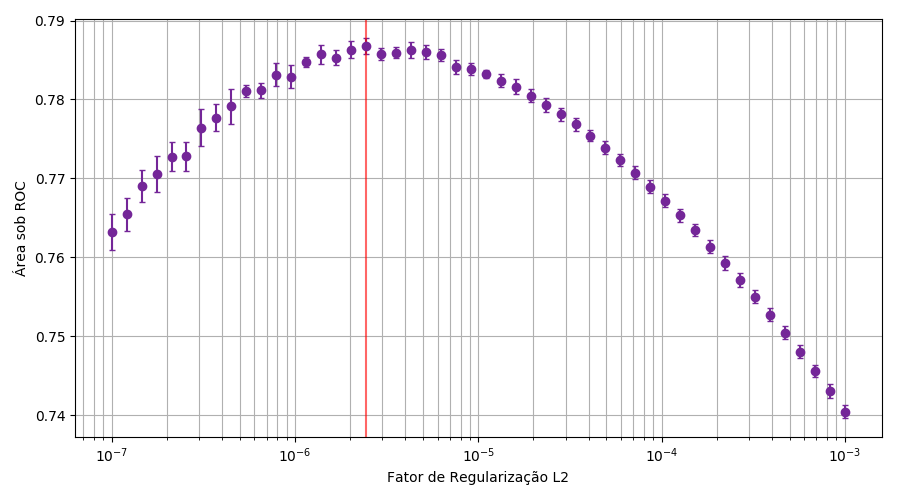
\includegraphics[scale=0.5]{svm_selecao.png}
    \caption{Seleção de hiperparâmetros de SVM - Etapa 2.}
    \label{fig:svm_selecao}
    \end{center}
}
\end{center}
\end{figure}

Uma vez selecionado os melhores hiperparâmetros, a Figura~\ref{fig:linear_roc_go} compara a curva ROC que caracteriza a
performance dos modelos treinandos tanto na primeira quanto na segunda etapa sob os dados de testes disponibilizados
por Go \textit{et al.}, a linha tracejada é utilizada como referência pois indica a performance de um classificador de
seleção aleatória.
Observamos na Figura ~\ref{fig:linear_roc_go} que os modelos da etapa 1, treinados com os dados do Sentiment140,
obtiveram resultados semelhantes entre si e consideravelmente superiores aos classificadores da segunda etapa, treinados
com base coletada neste trabalho, dentre os modelos da segunda etapa SVM se sobressaiu em relação ao Naïve Bayes.

A Figura~\ref{fig:linear_roc_semeval}, por sua vez, apresenta a curva ROC dos modelos quando aplicados nos dados
manualmente anotados coletados do SemEval.
O comportamento dos classificadores nesta base de dados se assemelha ao observado anteriormente, porém, neste caso a
performance dos classificadores de SVM e Naïve Bayes da segunda etapa praticamente se igualaram.

\begin{figure}
\begin{center} {
    \begin{center}
    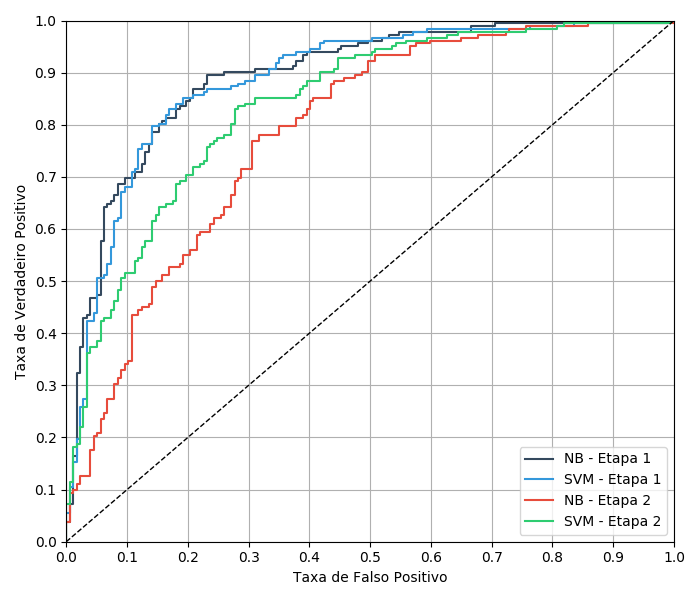
\includegraphics[scale=0.5]{linear_roc_go.png}
    \caption{Curva ROC dos modelos aplicados aos dados de teste do Sentiment140.}
    \label{fig:linear_roc_go}
    \end{center}
}
\end{center}
\end{figure}

\begin{figure}
\begin{center} {
    \begin{center}
    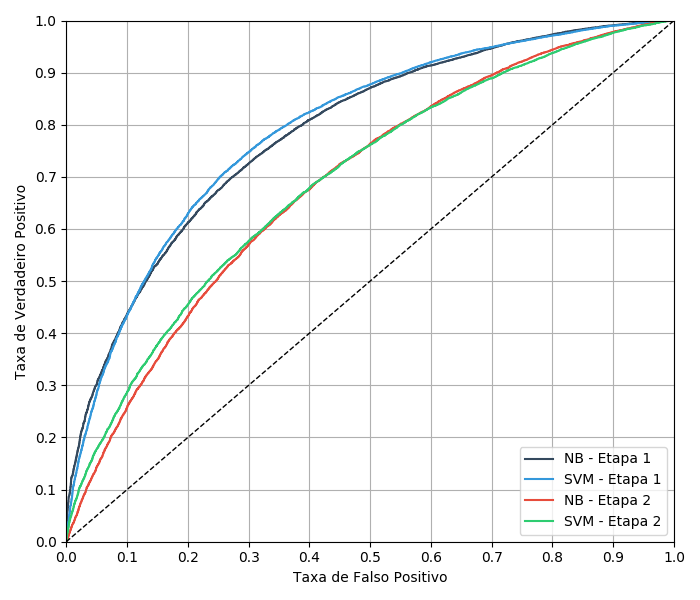
\includegraphics[scale=0.5]{linear_roc_semeval.png}
    \caption{Curva ROC dos modelos aplicados aos dados de teste do SemEval.}
    \label{fig:linear_roc_semeval}
    \end{center}
}
\end{center}
\end{figure}

Observa-se que os modelos treinados pelo conjunto de dados de anotação ruidosa disponibilizados por Go
\textit{et al.} apresentou desempenho consideravelmente melhor nos dois conjuntos de testes.
Desta maneira, se percebe que o processo de anotação dos dados foi mais ruidoso do que o apresentado pelo Sentiment140.

Uma hipótese a ser feita é que evoluções no idioma e na plataforma durante o intervalo entre a criação de ambas as
bases anotadas por supervisão distante tenha dificultado este processo, visto que a desenvolvida por Go \textit{et al.}
foi coletada em 2009, e a base de treinamento coletada para este trabalho conta com \textit{tweets} de 2017.
Constatou-se, por exemplo, que a base desenvolvida neste trabalho apresentou 1,1 milhões de palavras únicas após o
processo de tokenização, enquanto os dados de treinamento do Sentiment140 contam com 330 mil palavras únicas.

Outro fator relevante para definição de ruído no processo de anotação é a escolha dos \textit{emoticons}.
Neste trabalho, além dos \textit{emoticons} utilizados pelo Sentiment140, os \textit{emoticons} mais frequentes nos
dados foram selecionados para classificação manual.
A escolha de \textit{emoticons} de maneira a atingir maior correlação com as classes pode ser uma solução para reduzir
a diferença de performance dos modelos entre os resultados de treinamento e os resultados de teste.

Apesar dos resultados obtidos na base de treinamento anotada para este trabalho serem inferiores aos apresentados pelos
classificadores treinados com a base disponibilizada por Go \textit{et al.}, a técnica de supervisão distante por
\textit{emoticons} para anotação ruidosa de mensagens de redes sociais se mantém como boa alternativa ao processo
custoso de anotação manual.

A Tabela~\ref{tab:linear_perf} resume os resultados dos modelos treinados na primeira e na segunda etapas quando
aplicados sob ambos os conjuntos de testes.
Ressalta-se nesta tabela que os resultados dos classificadores treinados na segunda etapa foram consideravelmente
inferiores aos da primeira fase e que os algoritmos de Naïve Bayes e SVM apresentaram resultados semelhantes em
praticamente todas as situações, com exceção dos classificadores da segunda etapa aplicados na pequena base de teste
do Sentiment140.
O ponto de operação dos modelos foi escolhido de maneira a maximizar o índice SP.
É válido lembrar que a acurácia é uma métrica inconsistente quando consideras bases de testes com classes
desbalanceadas, como é o caso da base de \textit{tweets} coletados dos SemEval, sendo a área sob a curva ROC, AUC, ou o
índice SP, melhores opções para comparação destes casos.

% AUC -> CalibratedClassifier
% Acurácia, SP -> treshold: ponto de maior SP
\begin{table}[h]
    \begin{center}
        \begin{tabular}{ |l|l|l|r|r|r| }
            \hline
            \textbf{Dados de teste} & \multicolumn{2}{|c|}{\textbf{Modelo}}  & \textbf{Acurácia} & \textbf{AUC} & \textbf{SP} \\ \hline
            \multirow{4}{*}{Sentiment140} & \multirow{2}{*}{Etapa 1} & NB  & 83,3\% & 0,893 & 0,831 \\ \cline{3-6}
                                          &                          & SVM & 83,0\% & 0,887 & 0,830 \\ \cline{2-6}
                                          & \multirow{2}{*}{Etapa 2} & NB  & 73,3\% & 0,785 & 0,732 \\ \cline{3-6}
                                          &                          & SVM & 77,7\% & 0,839 & 0,776 \\ \hline
            \multirow{4}{*}{SemEval}      & \multirow{2}{*}{Etapa 1} & NB  & 70,9\% & 0,786 & 0,713 \\ \cline{3-6}
                                          &                          & SVM & 72,8\% & 0,791 & 0,724 \\ \cline{2-6}
                                          & \multirow{2}{*}{Etapa 2} & NB  & 64,9\% & 0,688 & 0,639 \\ \cline{3-6}
                                          &                          & SVM & 64,2\% & 0,693 & 0,640 \\ \hline
        \end{tabular}
        \caption{Resultados obtidos pelos classificadores treinados nas diferentes bases de dados e operados com limiar de decisão escolhido de maneira a maximizar o índice SP.}
        \label{tab:linear_perf}
    \end{center}
\end{table}

\section{Terceira Etapa}

A terceira fase do projeto visa a reproduzir redes neurais convolucionais aplicadas a texto e comparar seu desempenho
a algoritmos de aprendizado de máquina consolidados no processamento de linguagem natural, como presentes na etapa
anterior.
Neste estágio, as redes foram treinadas com dados provindos da base anotada por supervisão distante, mesmos dados
utilizados para treinamento dos algoritmos de Naïve Bayes e \textit{Support Vector Machines} da segunda etapa.
Após feita a seleção dos hiperparâmetros, o modelo é comparado aos treinados na segunda etapa com base no seu
desempenho obtido na base de testes disponibilizada pelas conferências SemEval.

Foram variados diversos hiperparâmetros, são eles: número de camadas, número de filtros convolucionais por camada,
tamanho dos filtros convolucionais, tamanho do filtro de \textit{pooling}.
Outros hiperparâmetros como: fator de regularização $L_{2}$ e probabilidade de Dropout foram mantidos fixos em
respectivamente $10^{-3}$ e $0,5$.
O valor escolhido de $\epsilon$, fator que define a estabilidade no treinamento, foi $10^{-3}$, o qual foi selecionado
após a análise de algumas curvas de treinamento.

A escolha dos hiperparâmetros foi feita de maneira a maximizar a área sob a curva ROC nos dados de validação.
A Tabela~\ref{tab:cnn_selection} lista os resultados obtidos por cada configuração treinada.

% apos treino coletar a auc de todos modelos (nos dados de treinamento mesmo), anotar valores na tabela
\begin{table}[h]
    \begin{center}
        \begin{tabular}{| >{\centering\arraybackslash}m{2.5cm} | >{\centering\arraybackslash}m{2.5cm} | >{\centering\arraybackslash}m{2.5cm} | >{\centering\arraybackslash}m{2.5cm}| c |}
        \hline
        \multicolumn{4}{|c|}{\textbf{Hiperparâmetros}} & \textbf{Resultado} \\ \hline
        \textbf{Número de Camadas} & \textbf{Número Filtros Conv.} & \textbf{Tamanho Filtros Conv.} & \textbf{Tamanho Filtros Pooling} & \textbf{AUC} \\ \hline
        \multirow{12}{*}{1} & \multirow{6}{*}{100} & \multirow{3}{*}{2} & 2 & 0,7637 \\ \cline{4-5}
                            &                      &                    & 3 & 0,7635 \\ \cline{4-5}
                            &                      &                    & 5 & 0,7636 \\ \cline{3-5}

                            &                      & \multirow{3}{*}{3} & 2 & 0,7677 \\ \cline{4-5}
                            &                      &                    & 3 & 0,7682 \\ \cline{4-5}
                            &                      &                    & 5 & 0,7667 \\ \cline{2-5}

                            & \multirow{6}{*}{200} & \multirow{3}{*}{2} & 2 & 0,7648 \\ \cline{4-5}
                            &                      &                    & 3 & 0,7616 \\ \cline{4-5}
                            &                      &                    & 5 & 0,7621 \\ \cline{3-5}

                            &                      & \multirow{3}{*}{3} & 2 & 0,7666 \\ \cline{4-5}
                            &                      &                    & 3 & 0,7687 \\ \cline{4-5}
                            &                      &                    & 5 & 0,7682 \\ \cline{1-5}

        \multirow{12}{*}{2} & \multirow{6}{*}{100} & \multirow{3}{*}{2} & 2 & 0,7604 \\ \cline{4-5}
                            &                      &                    & 3 & 0,7604 \\ \cline{4-5}
                            &                      &                    & 5 & 0,7598 \\ \cline{3-5}

                            &                      & \multirow{3}{*}{3} & 2 & 0,7677 \\ \cline{4-5}
                            &                      &                    & 3 & 0,7678 \\ \cline{4-5}
                            &                      &                    & 5 & 0,7680 \\ \cline{2-5}

                            & \multirow{6}{*}{200} & \multirow{3}{*}{2} & 2 & 0,7618 \\ \cline{4-5}
                            &                      &                    & 3 & 0,7622 \\ \cline{4-5}
                            &                      &                    & 5 & 0,7617 \\ \cline{3-5}

                            &                      & \multirow{3}{*}{3} & 2 & 0,7684 \\ \cline{4-5}
                            &                      &                    & 3 & 0,7648 \\ \cline{4-5}
                            &                      &                    & 5 & 0,7667 \\ \cline{1-5}

        \end{tabular}
    \caption{Seleção de hiperparâmetros de CNN.}
    \label{tab:cnn_selection}
    \end{center}
\end{table}

De acordo com a Tabela~\ref{tab:cnn_selection}, podemos observar que os resultados obtidos foram muito próximos
entre si, apresentando diferença de 0,0089 de área de curva ROC entre a melhor e a pior configuração quando aplicados
aos dados de validação.
O conjunto de parâmetros com melhor desempenho foram: 1 camada composta por 200 filtros
convolucionais de tamanho 3, seguida de uma camada de \textit{pooling} com filtro de tamanho 3.
Analisando os resultados das diferentes configurações, observamos que filtros convolucionais de tamanho 3 obtiveram
melhores resultados.
Dentre os outros parâmetros variados não se destacou nenhum valor consistentemente melhor dentre os valores testados.

A Figura~\ref{fig:cnn_learning_curve} mostra a curva de treinamento do modelo com a melhor configuração de hiperparâmetros.
Essa figura mostra a evolução do valor da função custo, presente no eixo vertical, tanto sob os dados de treinamento
quanto de validação na medida em que o classificador é treinado.
Nesta figura, se observa que o ponto de menor valor de função custo de validação é obtido na oitava época.
Sendo assim, os pesos referentes a oitava época foram selecionados para compor o modelo.

\begin{figure}
\begin{center} {
    \begin{center}
    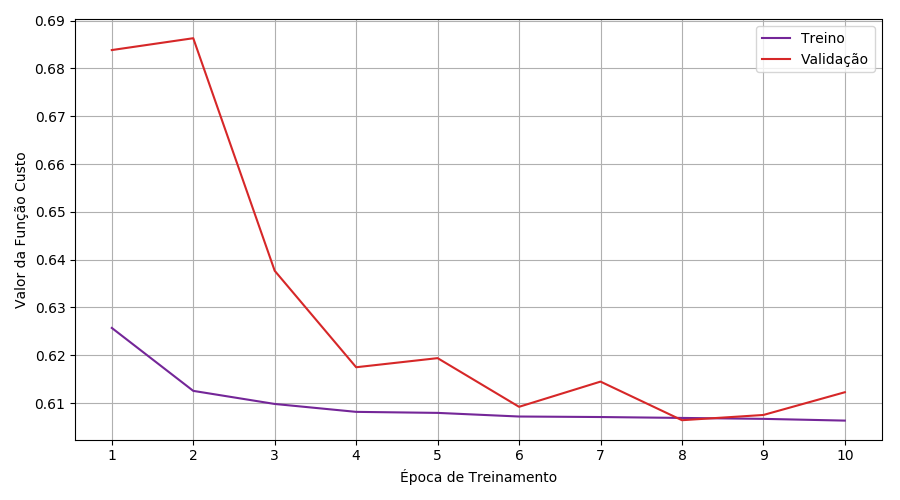
\includegraphics[scale=0.5]{cnn_learning_curve.png}
    \caption{Curva de treinamento da rede neural convolucional.}
    \label{fig:cnn_learning_curve}
    \end{center}
}
\end{center}
\end{figure}

Uma vez selecionados os hiperparâmetros da rede neural convolucional, a Figura~\ref{fig:all_roc_semeval} apresenta a
curva ROC comparativa entre os modelos que foram treinados a partir da base de dados com anotação ruidosa formada por
este trabalho.
Nessa figura são apresentadas as curvas ROC dos modelos quando aplicados a base de testes formada por \textit{tweets}
fornecido pelas conferências SemEval e destaca-se que o modelo de redes neurais convolucionais superou os resultados
obtidos por Naïve Bayes e SVM, principalmente nos limiares de decisão que correspondem a menor taxa de falsos positivos.

A Tabela~\ref{tab:all_compara} resume os resultados destes classificadores, novamente considerando que o limiar de
decisão foi selecionado de maneira a maximizar o índice SP.
Assim como podemos observar na Figura~\ref{fig:all_roc_semeval} a rede convolucional apresentou maior área sob a curva
ROC quando comparada aos modelos tradicionalmente aplicados a texto.

\begin{figure}
\begin{center} {
    \begin{center}
    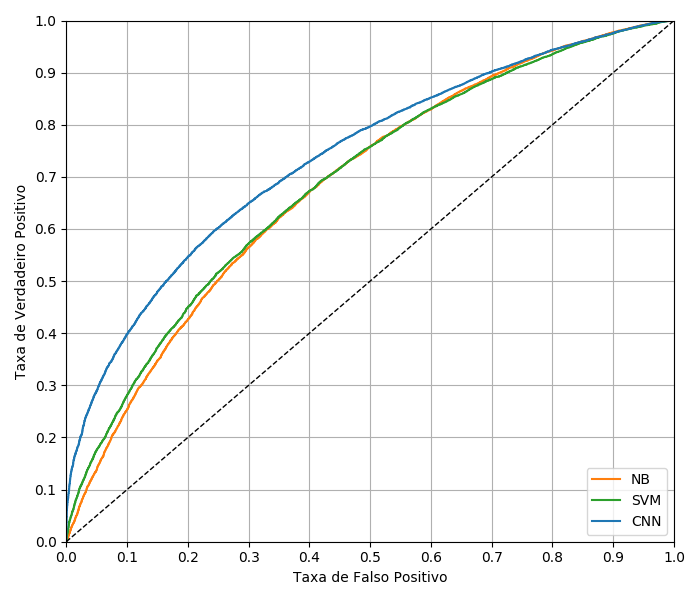
\includegraphics[scale=0.5]{all_roc_semeval.png}
    \caption{Curva ROC comparativa dos modelos treinados por dados de supervisão distante.}
    \label{fig:all_roc_semeval}
    \end{center}
}
\end{center}
\end{figure}

\begin{table}[h]
    \begin{center}
        \begin{tabular}{| l | r | r |}
        \hline
        \textbf{Algoritmo} & \textbf{AUC} & \textbf{SP} \\ \hline
        Naïve Bayes & 0,688 & 0,639 \\ \hline
        \textit{Support Vector Machine} & 0,693 & 0,640 \\ \hline
        Redes Convolucionais & 0,738 & 0,675 \\ \hline
        \end{tabular}
        \caption{Comparação dos algoritmos treinados por dados de supervisão distante.}
        \label{tab:all_compara}
    \end{center}
\end{table}

Pode se observar que a utilização de redes neurais convolucionais em conjunto com representações obtidas por
Word2Vec propiciou resultados melhores do que os obtidos com modelos tradicionais, como Naïve Bayes e
\textit{Support Vector Machines} sobre representações \textit{one-hot} dos textos.
Ressalta-se que a representação Word2Vec utilizada foi desenvolvida a partir de notícias.
O treinamento de modelos próprios para o meio no qual serão empregados, neste caso, \textit{tweets}, pode melhorar o
desempenho do classificador a ser utilizado.
